\documentclass[a4paper,12pt]{article}
\usepackage[utf8x]{inputenc}
\usepackage[swedish]{babel}
\usepackage[T1]{fontenc}
\usepackage{graphicx}
\usepackage{placeins}
\usepackage{bmpsize}
\usepackage{amsfonts, amsmath, amssymb}
\usepackage{ccfonts,euler}
\usepackage{wrapfig}
\usepackage{multirow}
\usepackage{caption}
\usepackage{enumerate}
\usepackage{comment}
\usepackage[includeheadfoot,margin=1.1in]{geometry}
\usepackage{listings}
\usepackage{color}
\usepackage{verbatim}

\definecolor{dkgreen}{rgb}{0,0.6,0}
\definecolor{gray}{rgb}{0.5,0.5,0.5}
\definecolor{mauve}{rgb}{0.58,0,0.82}

\lstset{frame=tb,
  language=Python,
  aboveskip=3mm,
  belowskip=3mm,
  showstringspaces=false,
  columns=flexible,
  basicstyle={\small\ttfamily},
  numbers=none,
  numberstyle=\tiny\color{gray},
  keywordstyle=\color{blue},
  commentstyle=\color{dkgreen},
  stringstyle=\color{mauve},
  breaklines=true,
  breakatwhitespace=true,
  tabsize=3,
  literate={å}{{\r a}}1 {ö}{{\"o}}1 {ä}{{\"a}}1 {Å}{{\r A}}1 {Ö}{{\"O}}1 {Ä}{{\"A}}1
}

\oddsidemargin -15mm
\evensidemargin -15mm
\marginparwidth 5mm
\topmargin -28mm
\textheight 282mm
\textwidth 190mm
\headheight 4mm
\headsep 4mm

\sloppy

\newcounter{iii}\setcounter{iii}{0}
\def\i{\bigskip\noindent\refstepcounter{iii}\textbf{\arabic{iii}.} }
%\def\iotst#1{\par \smallskip \mbox{}\refstepcounter{iii}\hspace*{#1}\textbf{\arabic{iii}.}}
\newcounter{pun}[iii]
\def\pu{\refstepcounter{pun}{\bf(\alph{pun})}\ }
\def\Pu{\par\noindent\mbox{}\refstepcounter{pun}{\phantom{\textbf{\arabic{iii}.}}\hspace{0.2mm}\bf(\alph{pun})}\ }

\def\ext{\subsection*{Extrauppgifter}}

\title{Programmering, Nao - Extrauppgifter}
\date{29 juli}

\makeatletter
\let\newtitle\@title
\let\newdate\@date
\makeatother
\begin{document}

  \renewcommand*\rmdefault{ppl}\normalfont\upshape
\pagestyle{empty}
\large
\section*{\newdate\ \  \newtitle}

\i

Valentina tycker om choklad. Hon har därför alltid en öppnad chokladkartong i skafferiet. När den tar slut köper hon i hemlighet en ny och låtsas som ingenting. Valentinas bror Danil, som är misstänksam av naturen, förundras över att den där kartongen aldrig tar slut. Därför börjar han vid varje besök att räkna antalet chokladbitar som är kvar. Skriv ett program som, givet hans observationer, beräknar det minsta antalet nya kartonger Valentina måste ha köpt under perioden. 

\textbf{Indata}

På första raden följer en rad med $N$ heltal (lika många heltal som observationer), där heltalen motsvarar antalet chokladbitar i asken (mellan 1 och 100) vid varje observation, i den ordning de görs.

\textbf{Utdata}

Programmet ska skriva ut ett heltal: det minsta antal nya kartonger Valentina bevisligen måste ha köpt under perioden.


\textbf{Körningsexempel:}
\begin{lstlisting}
Observationer ? 17 15 16 16 18 17 14 12 13 9
Valentina måste åtminstone ha köpt 3 chokladaskar.

Observationer ? 100 67 56 73 54 98 83 32 67 34 21 21 1 54 67 45 93 86 35 63 2
Valentina måste åtminstone ha köpt 7 chokladaskar.

Observationer ? 88 79 65 61 57 32 87 54 98 21 56 56 56 73
Valentina måste åtminstone ha köpt 4 chokladaskar.
\end{lstlisting}

% Lösningsförslag:
% (1) observationer = [17, 15, 16, 16, 18, 17, 14, 12, 13, 9]
% (2) observationer = [100,67,56,73,54,98,83,32,67,34,21,21,1,54,67,45,93,86,35,63,2]
% (3) observationer = [88, 79, 65, 61, 57, 32, 87, 54, 98, 21, 56, 56, 56, 73]
% antal_observationer = len(observationer)
% antal_chokladaskar = 0
% for i in range(antal_observationer - 1):
%     if observationer[i+1] > observationer[i]:
%         antal_chokladaskar += 1
% print("antal chokladaskar: ", antal_chokladaskar)


\i

Leonid kandiderar till ordförandeposten i matematiksällskapet och vill inte riskera att förlora omröstningen. Han har lyckats få reda på vilken kandidat varje medlem tänker rösta på och tänker helt enkelt muta ett antal medlemmar så att de röstar på honom istället. Skriv ett program som beräknar hur många röster som måste köpas (d.v.s. medlemmar som behöver mutas) för att Leonid ska vinna omröstningen. För att vinna krävs att man får fler röster än var och en av de andra kandidaterna.

\textbf{Indata}
Först ska man mata in antal kandidater ($1 \le n \le 20$). Sedan ska man mata in $n$ heltal (mellan 0 och 1000): antalet röster varje kandidat skulle få utan mutor. Det första talet anger Leonids röster.

\textbf{Utdata}

Programmet ska skriva ut ett heltal: det minsta antalet röster som behöver köpas för att Leonid ska få fler röster än var och en av de övriga kandidaterna.

\pagebreak
\textbf{Körningsexempel:}
\begin{lstlisting}
Antal kandidater ? 4
Röster som Leonid skulle fått utan mutor ? 2 
Röster som de andra skulle fått utan mutor ? 5 7 8
Leonid måste åtminstone köpa 5 röster.

Antal kandidater ? 6
Röster som Leonid skulle fått utan mutor ? 11
Röster som de andra skulle fått utan mutor ? 10 14 0 2 8
Leonid måste åtminstone köpa 2 röster.

Antal kandidater ? 9
Röster som Leonid skulle fått utan mutor ? 6
Röster som de andra skulle fått utan mutor ? 4 3 8 4 4 16 18 2
Leonid måste åtminstone köpa 8 röster.
\end{lstlisting}

%\textbf{Förklaring:} Leonid kan t.ex. köpa 3 röster som skulle tillfallit den fjärde kandidaten samt 2 röster som skulle tillfallit den tredje kandidaten. Då får han själv 7 röster medan övriga kandidater får 5 röster.

\begin{comment}
antal_kandidater = 9
Leonid_röster = 6
andras_röster = [4,3,8,4,4,16,18,2]

andras_röster.sort()
andras_röster.reverse()

antal_mutor = 0
while Leonid_röster <= andras_röster[0]:
    Leonid_röster += 1
    andras_röster[0] -= 1
    andras_röster.sort()
    andras_röster.reverse()
    antal_mutor += 1


print("Leonids röster: ", Leonid_röster)
print("De andras röster efter mutning: ", andras_röster)
print("Antal mutor Leonid måste köpa: ", antal_mutor)

\end{comment}

\i



I egyptisk matematik hade de så kallade heltalsreciprokerna

${\displaystyle {\frac {1}{1}},{\frac {1}{2}},{\frac {1}{3}},{\frac {1}{4}},...}$

särskild betydelse. Övriga bråk skrevs som summor av dessa tal, t.ex.

${\displaystyle {\frac {21}{20}}={\frac {1}{2}}+{\frac {1}{4}}+{\frac {1}{5}}+{\frac {1}{10}}}$

Skriv ett program som tar emot ett bråk (förkortat så långt som möjligt) och avgör om det kan skrivas som en sådan summa, under villkoren att bara de tio första heltalsreciprokerna (alltså t.o.m. 1/10) får användas, och att varje tal endast får användas en gång. Om det går ska programmet skriva ut de ingående termerna i summan, annars ska det skriva ut Omöjligt. Om det finns flera lösningar ska programmet skriva ut vilken som helst av dem.



\textbf{Två körningsexempel:}
\begin{lstlisting}
Täljare ? 67
Nämnare ? 60
Termer: 1/2 1/4 1/5 1/6

Täljare ? 2
Nämnare ? 5
Omöjligt
\end{lstlisting}

\begin{comment}
#!/usr/bin/python
# -*- coding: utf-8 -*-
# Nämnarna till våra bråk som vi får bilda summor av.
namnarna = [1,2,3,4,5,6,7,8,9,10]
# Täljarna till våra bråk, när vi har förlängt alla till gemensam nämnare.
# Alla initieras till 0. Om en täljare senare fortfarande är 0, så betyder det
# att det bråket inte är kompatibelt med bråket som användaren har matat in.
taljarna = [0] * len(namnarna)
# Täljaren som användaren ska ange.
taljare = input("Täljare ? ")
# Nämnaren som användaren ska ange.
namnare = input("Nämnare ? ")

# Sparar talföljden av bråk som kunde bilda det önskade bråket.
# Om längden på strängen frotfarande är 0 vid programmets slut
# så betyder det att uppgiften var omöjlig.
successful = ""



def rek(frac, sequence, i):
    """
    Vår rekursiva funktion som ska lösa problemet.
    frac: Täljaren till det bråk vi för tillfället har. Nämnaren behöver vi inte
    hålla reda på eftrsom den är densamma för alla.
    sequence: Talföljden av bråk som ledde fram till vårt nuvarande.
    int i: Indexet för det bråk vi är på och ska testa att lägga till på talföljden.
    """
    global successful

    # Om vår täljare är = den önskade täljaren så har vi lyckats.
    if frac == taljare:
	# Sparar talföljden som ledde fram till svaret.
	successful = sequence
	# Returnerar, det är ju dumt att lägga till bråk på ett bråk som redan är rätt.
	return

    # Om vårt bråk redan är större än det önskade, så behöver vi ju inte fortsätta
    # att lägga till bråk på talföljden.
    elif frac > taljare:
        return

    # Eller om vi redan har avverkat alla bråk, då ska man avbryta.
    elif i >= len(namnarna):
	return



    # Om detta bråk är kompatibelt med vårt bråk.
    if taljarna[i] != 0: 
	# Lägger till bråket på talföljden.
	rek(frac+taljarna[i], sequence+"1/"+str(namnarna[i])+" ", i+1)

    # Bara för att bråket är kompatibelt, så behöver ju inte det betyda att det ska ingå i den korrekta talfölden.
    # Att testa att inte ta med bråket är minst lika viktigt.
    rek(frac, sequence, i+1)






# Loopar igenom alla bråk och kollar om de funkar tillsammans med det inmatade bråket.
for i in range(len(namnarna)):
    # Om den inmatade nämnaren är jämnt delbar med nuvarande bråks nämnare, så är bråket kompatibelt.
    if namnare % namnarna[i] == 0:
	# Om vi förlänger bråket till det inmatade bråkets nämnare, så kommer alla bråken såklart få samma nämnare.
        # Det enda som skiljer sig är täljaren. Alltså behöver vi bara hålla koll på täljaren som vi ska addera. 
	taljarna[i] = namnare/namnarna[i]
    # Om inte så förblir täljaren till bråket 0, vilket indikerar att bråket inte är kompatibelt.

print(taljarna)
# Nu ska vi hitta talföljden, det enda vi behöver göra är att addera ihop våra täljare som vi har tagit fram
# i loopen ovan tills vi får samma täljare som användaren har matat in. Lätt som en plätt.
# Vi börjar så klart med 0 (vi har inte adderat några täljare ännu), en tom sträng (inga tal ingår i talföljden än så länge)
# och vi ska börja att testa med det första bråket (täljaren) som har index 0.
rek(0, "", 0)




# Om strängen som har svaret inte har längden 0, så finns det ett svar.
if len(successful):
    print("Termer: " + successful)
# Om den är 0 så var visst uppgiften omöjlig.
else:
    print("Omöjligt")
\end{comment}

\pagebreak

\i

\begin{figure}[!ht]
\centering
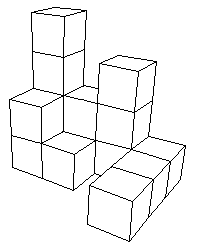
\includegraphics[width=0.2\textwidth]{begransningsarea.png}
\caption{}
\label{fig:begransningsarea}
\end{figure}

Betrakta den tredimensionalla figuren ovan. Den är ihopsatt av ett antal $1\times1\times1$ kuber i ett 3d-rutnät. Vi begränsar oss till figurer som har staplar fästa i ''marken'', så ingen kub har luft under sig. 

Figurens volym är förstås enkel att beräkna, men här är vi intresserade av dess begränsningsarea, d.v.s. antalet $1\times1$ kvadrater som är synliga utifrån (inklusive underifrån). Skriv ett program som beräknar detta, givet beskrivningen av en figur.
Figurens basarea kan maximalt vara $50\times50$, och staplarnas höjd är maximalt 50. 


\textbf{Körningsexempel:}

\begin{lstlisting}
Höjdinformation ? 
4 2 3 1
2 1 0 1
0 0 0 1
Begränsningsarean blir totalt: 54


Höjdinformation ? 
1 3
4 5
Begränsningsarean blir totalt: 42


Höjdinformation ? 
4  6  2  7 8  3 5 12 9
5  7  6  2 4  3 1 4  7
3  2  6  3 9  6 5 3  8
10 25 13 7 7  0 0 1  9
4  36 12 4 18 3 5 0  0
Begränsningsarean blir totalt: 658
\end{lstlisting}
\begin{comment}
(1) kuber = [[4, 2, 3, 1],[2, 1, 0, 1],[0, 0, 0, 1]]
(2) kuber = [[1,3],[4,5]]
(3) kuber = [[4, 6, 2, 7, 8, 3, 5, 12, 9], [5, 7, 6, 2, 4, 3, 1, 4, 7], [3, 2, 6, 3, 9, 6, 5, 3, 8], [10, 25, 13, 7, 7, 0, 0, 1, 9], [4, 36, 12, 4, 18, 3, 5, 0, 0]]

antal_kuber = 0
antal_sidor_bredvid_annan_kub = 0
for i in range(len(kuber)):
    for j in range(len(kuber[i])):
        if kuber[i][j] != 0:
            antal_kuber += kuber[i][j]
            antal_sidor_bredvid_annan_kub += (kuber[i][j] - 1)*2
            if i < len(kuber)-1:
                if kuber[i+1][j] != 0:
                    if kuber[i+1][j] >= kuber[i][j]:
                        antal_sidor_bredvid_annan_kub += kuber[i][j]
                    else:
                        antal_sidor_bredvid_annan_kub += kuber[i+1][j]
            if i > 0:
                if kuber[i-1][j] != 0:
                    if kuber[i-1][j] >= kuber[i][j]:
                        antal_sidor_bredvid_annan_kub += kuber[i][j]
                    else:
                        antal_sidor_bredvid_annan_kub += kuber[i-1][j]
            if j < len(kuber[i])-1:
                if kuber[i][j+1] != 0:
                    if kuber[i][j+1] >= kuber[i][j]:
                        antal_sidor_bredvid_annan_kub += kuber[i][j]
                    else:
                        antal_sidor_bredvid_annan_kub += kuber[i][j+1]
            if j > 0:
                if kuber[i][j-1] != 0:
                    if kuber[i][j-1] >= kuber[i][j]:
                        antal_sidor_bredvid_annan_kub += kuber[i][j]
                    else:
                        antal_sidor_bredvid_annan_kub += kuber[i][j-1]

print("Begränsningsarea: ", antal_kuber*6 - antal_sidor_bredvid_annan_kub)
\end{comment}

\pagebreak

\i 

\begin{figure}[!ht]
\centering
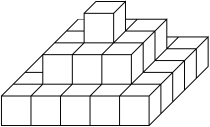
\includegraphics[width=0.3\textwidth]{pyramid.png}
\caption{Denna pyramid med höjden 3 innehåller 35 stenblock. Cheopspyramiden i Egypten har höjden 210.}
\label{fig:begransningsarea}
\end{figure}

När man ska inleda ett större projekt, exempelvis bygga en pyramid, är det bäst att tänka efter en gång extra. Du ska skriva ett program som beräknar hur hög pyramid man kan bygga om man har tillgång till ett visst antal stenblock.

Vi antar att pyramiden är kompakt, d.v.s. det finns inga hålrum inuti. Vidare byggs den enligt principen i figuren ovan. Varje lager är alltså kvadratiskt med en sidlängd som är två block mindre än det underliggande lagrets. Det översta lagret består alltid av ett ensamt block.

Programmet ska fråga efter antalet tillgängliga block (högst hundra miljoner) och skriva ut höjden (i block räknat) för den största pyramid som kan byggas. Det gör ingenting om det blir block över, men det får inte saknas ett enda block.

\textbf{Körningsexempel:}
\begin{lstlisting}
Antal block ? 83  
Höjd: 3 

Antal block ? 165
Höjd: 5

Antal block ? 456  
Höjd: 7 

Antal block ? 12347930 
Höjd: 210
\end{lstlisting}

\begin{comment}
(exempel) antal_stenblock = 35 # = 1*1+3*3+5*5, höjd = 3
(1) antal_stenblock = 83 # = 1*1+3*3+5*5+48, höjd = 3
(2) antal_stenblock = 165 # = 1*1+3*3+5*5+7*7+9*9, höjd = 5
(3) antal_stenblock = 456 # = 1*1+3*3+5*5+7*7+9*9+11*11+13*13+1, höjd = 7
(4) antal_stenblock = 12347930

antal_stenblock = int(input("Antal stenblock: "))

antal_stenblock_använda = 0
höjd = 0
while True:
    antal_stenblock_till_nästa_höjd = (höjd*2 + 1)**2
    if antal_stenblock_till_nästa_höjd <= antal_stenblock-antal_stenblock_använda:
        antal_stenblock_använda += antal_stenblock_till_nästa_höjd
        höjd += 1
    else:
        break
print(höjd)
\end{comment}

\pagebreak

\i 

En sfinx är en varelse med ett lejons kropp och en människas huvud. Liknande kombinationer återfinns i andra kulturer, t.ex. faunen (get+människa) och gripen (örn+lejon). Man skulle kunna tro att den ringa förekomsten av sådana arter i naturen beror på viss svårighet i fortplantningen, men i denna uppgift antar vi raka motsatsen.

Med hänvisning till genetikens lagar antar vi att när två kombinationsvarelser parar sig så ärver avkomman framkroppen från den ena föräldern och bakkroppen från den andra. En grodmus som parar sig med en fiskhöna kan alltså ge upphov till antingen en grodhöna eller en fiskmus.

Skriv ett program som, givet en grupp kombinationsvarelser (somliga hannar och andra honor) beräknar antalet olika arter som kan existera i nästa generation om alla par av hanne-hona antas få ungar. Svaret ska också inkludera de arter som ingår i den ursprungliga gruppen.

Programmet ska fråga efter antalet hannar och vilken art varje hanne tillhör, samt likadant för honorna. Arten anges som en sträng med två bokstäver (valda bland A-Z), där första bokstaven beskriver framkroppen och andra bokstaven bakkroppen (t.ex. ML för människolejon). Programmet ska skriva ut det totala antalet olika arter som kan finnas när parning har skett. Observera att ordningen på bokstäverna spelar roll – MF och FM är olika arter.


\textbf{Körningsexempel:}
\begin{lstlisting}
Antal hannar ? 2  
Hanne 1 ? ML  
Hanne 2 ? FG 
Antal honor ? 3 
Hona 1 ? VM 
Hona 2 ? FM 
Hona 3 ? VF 
Antal arter: 11 


Antal hannar ? 5 
Hanne 1 ? HM  
Hanne 2 ? FB 
Hanne 3 ? OH 
Hanne 4 ? GO 
Hanne 5 ? SO 
Antal honor ? 6
Hona 1 ? BF 
Hona 2 ? GM 
Hona 3 ? VM 
Hona 4 ? VF 
Hona 5 ? FG 
Hona 6 ? HM 
Antal arter: 36
\end{lstlisting}

\begin{comment}
alla_varelser = [None]

hannar = []
antal_hannar = int(input("Antal hannar: "))
for i in range(antal_hannar):
    hane = input("Skriv in hane nr%s : " %(i+1))
    hannar.append(hane)
    for varelse in alla_varelser:
        if varelse == hane:
                break
        if varelse == alla_varelser[-1]:
            alla_varelser.append(hane)
honor = []
antal_honor = int(input("Antal honor: "))
for i in range(antal_honor):
    hona = input("Skriv in hona nr%s : " %(i+1))
    honor.append(hona)
    for varelse in alla_varelser:
        if varelse == hona:
                break
        if varelse == alla_varelser[-1]:
            alla_varelser.append(hona)
   
for hane in hannar:
    for hona in honor:
        for varelse in alla_varelser:
            if varelse == hane[0]+hona[1]:
                break
            if varelse == alla_varelser[-1]:
                alla_varelser.append(hane[0]+hona[1])
        for varelse in alla_varelser:
            if varelse == hona[0]+hane[1]:
                break
            if varelse == alla_varelser[-1]:
                alla_varelser.append(hona[0]+hane[1])
#alla_varelser.pop(0) # Kan använda .pop(0) eller del 
del alla_varelser[0]
print(alla_varelser)
print(len(alla_varelser))
\end{comment}

\pagebreak

\i

\begin{figure}[!ht]
\centering
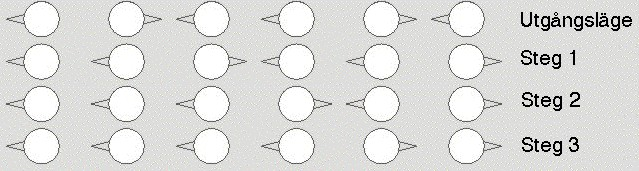
\includegraphics[width=0.8\textwidth]{soldater.jpg}
\caption{Uppställning av soldater}
\label{fig:soldater}
\end{figure}

Ett antal soldater står på ett led alla vända mot furiren, när han ger ordern "höger om". Eftersom många av soldaterna har svårt att skilja på höger och vänster blir det mest slumpen som avgör åt vilket håll de vänder sig. Ett exempel visas på första raden i figuren ovan. De soldater som på så sätt hamnar ''öga mot öga'' med en granne förstår båda två att de vänt sig åt fel håll och gör därför helt om (180 grader), för att kanske hamna öga mot öga med den andra grannen. Denna procedur fortsätter (steg 1 och 2 i figuren) och upphör då inga soldater längre är vända mot varandra (steg 3).

\textbf{Indata}

En rad där varje tecken är antingen V eller H. Dessa anger åt vilket håll soldatens näsa pekar i utgångsläget. Maximalt 100 tecken. 

\textbf{Utdata}
Programmet ska skriva ut hur många steg som behövs från utgångsläget tills lugnet infinner sig.

\textbf{Körningsexempel:}
\begin{lstlisting}
Soldater? VHVVHV
Det behövs totalt 3 steg för att lugna soldaterna

Soldater? HVHVHVHHVHVHVHVVHHHHVHHVHVVVHHVHHVHVHVHVHVHVHHH
Det behövs totalt 24 steg för att lugna soldaterna
\end{lstlisting}

\begin{comment}
persons = input("Soldater? ")
count = 0 # antalet vändningar
while "HV" in persons: # så länge minst två soldater står bredvid varandra
    persons = persons.replace("HV", "VH") #vänd soldaterna
    count += 1
print(count)
\end{comment}

\end{document}